\documentclass{article}

\usepackage[a4paper,margin=1in]{geometry}
\usepackage{fancyhdr}
\usepackage{amsmath}
\usepackage{booktabs}
\usepackage{listings}
\usepackage{graphicx}

\pagestyle{fancy}
\fancyhf{}
\lhead{Programming Language: Assignment 2}
\rhead{Sui Qingyu (5090309011)}
\cfoot{\thepage}

\setlength\parskip{0.5em}

\lstset{numbers=left,
       numberstyle=\scriptsize,
       frame=lines,
       flexiblecolumns=false,
       language=C,
       basicstyle=\ttfamily\small,
       breaklines=true,
       extendedchars=true,
       escapechar=\%,
       texcl=true,
       showstringspaces=true,
       keywordstyle=\bfseries,
       tabsize=4}

\begin{document}
\section*{Problem 1}
\textbf{Q:} \textit{Rewrite the productions for Identifier and Float's non-terminals as right and left regular grammars.}

Identifier, left regular grammar:
\begin{align*}
i &\rightarrow l\ i' \\
i' &\rightarrow \epsilon\ |\ l\ i'\ |\ d\ i' \\
l &\rightarrow a\ |\ b\ |\ \dots\ |\ z\ |\ A\ |\ B\ |\ \dots\ |\ Z \\
d &\rightarrow 0\ |\ 1\ |\ \dots\ |\ 9
\end{align*}

Identifier, right regular grammar:
\begin{align*}
i &\rightarrow i'\ l\ |\ i\ d \\
i' &\rightarrow \epsilon\ |\ i'\ l\ |\ i\ d \\
l &\rightarrow a\ |\ b\ |\ \dots\ |\ z\ |\ A\ |\ B\ |\ \dots\ |\ Z \\
d &\rightarrow 0\ |\ 1\ |\ \dots\ |\ 9
\end{align*}

Float, left regular grammar:
\begin{align*}
f &\rightarrow i\ .\ i \\
i &\rightarrow d\ i' \\
i' &\rightarrow \epsilon\ |\ d\ i' \\
d &\rightarrow 0\ |\ 1\ |\ \dots\ |\ 9
\end{align*}

Float, right regular grammar:
\begin{align*}
f &\rightarrow i\ .\ i \\
i &\rightarrow i'\ d \\
i' &\rightarrow \epsilon\ |\ i'\ d \\
d &\rightarrow 0\ |\ 1\ |\ \dots\ |\ 9
\end{align*}

\section*{Problem 2}
\textbf{Q:} \textit{Develop 8 test cases for Clite's Lexer. Explain the purpose of each test case. Run the test cases and hand in the output as well as the test cases.}

The answer is in the tables below.

\begin{table}[hp]
\begin{center}
\begin{tabular}{|l|l|l|l|}
\hline
Input & Expected Output & Actual Output & Pass / Fail \\
\hline
bool i; & TokenType.Bool & bool & fail \\
 & TokenType.Identifier & Identifier i & \\
 & TokenType.Semicolon & & \\
\hline
\end{tabular}
\end{center}
\caption{Case 1}
\end{table}

\begin{table}[hp]
\begin{center}
\begin{tabular}{|l|l|l|l|}
\hline
Input & Expected Output & Actual Output & Pass / Fail \\
\hline
if (a $<$ b) a = b; & TokenType.If & if & fail \\
 & TokenType.LeftParen & & \\
 & TokenType.Identifier & & \\
 & TokenType.Less & & \\
 & TokenType.Identifier & & \\
 & TokenType.RightParen & & \\
 & TokenType.Identifier & & \\
 & TokenType.Assign & & \\
 & TokenType.Identifier & & \\
 & TokenType.Semicolon & & \\
\hline
\end{tabular}
\end{center}
\caption{Case 2}
\end{table}

\begin{table}[hp]
\begin{center}
\begin{tabular}{|l|l|l|l|}
\hline
Input & Expected Output & Actual Output & Pass / Fail \\
\hline
a $||$ b \&\& c & TokenType.Identifier & Identifier a & pass \\
 & TokenType.Or & $||$ & \\
 & TokenType.Identifier & Identifier b & \\
 & TokenType.And & \&\& & \\
 & TokenType.Identifier & Identifier c & \\
\hline
\end{tabular}
\end{center}
\caption{Case 3}
\end{table}

\begin{table}[hp]
\begin{center}
\begin{tabular}{|l|l|l|l|}
\hline
Input & Expected Output & Actual Output & Pass / Fail \\
\hline
a + b / c & TokenType.Identifier & Identifier a & pass \\
 & TokenType.Plus & + & \\
 & TokenType.Identifier & Identifier b & \\
 & TokenType.Divide & / & \\
 & TokenType.Identifier & Identifier c & \\
\hline
\end{tabular}
\end{center}
\caption{Case 4}
\end{table}

\begin{table}[hp]
\begin{center}
\begin{tabular}{|l|l|l|l|}
\hline
Input & Expected Output & Actual Output & Pass / Fail \\
\hline
-3.5 & TokenType.Minus & & fail \\
 & TokenType.Float & & \\
\hline
\end{tabular}
\end{center}
\caption{Case 5}
\end{table}

\begin{table}[hp]
\begin{center}
\begin{tabular}{|l|l|l|l|}
\hline
Input & Expected Output & Actual Output & Pass / Fail \\
\hline
3.5 & TokenType.Float & & fail \\
\hline
\end{tabular}
\end{center}
\caption{Case 6}
\end{table}

\begin{table}[hp]
\begin{center}
\begin{tabular}{|l|l|l|l|}
\hline
Input & Expected Output & Actual Output & Pass / Fail \\
\hline
a != b & TokenType.Float & & fail \\
\hline
\end{tabular}
\end{center}
\caption{Case 7}
\end{table}

\begin{table}[hp]
\begin{center}
\begin{tabular}{|l|l|l|l|}
\hline
Input & Expected Output & Actual Output & Pass / Fail \\
\hline
while (a $<$ b) a = a + 1; & TokenType.While & while & fail \\
 & TokenType.LeftParen & & \\
 & TokenType.Identifier & & \\
 & TokenType.Less & & \\
 & TokenType.Identifier & & \\
 & TokenType.RightParen & & \\
 & TokenType.Identifier & & \\
 & TokenType.Assign & & \\
 & TokenType.Identifier & & \\
 & TokenType.Plus & & \\
 & TokenType.Int & & \\
\hline
\end{tabular}
\end{center}
\caption{Case 8}
\end{table}

\section*{Problem 3}
\textbf{Q:} \textit{Write down the equivalent concrete grammar in BNF for the following EBNF.}\\

\textit{a)} $A \rightarrow x\ (\ y\ |\ z\ )$

The answer is:
\begin{align*}
A &\rightarrow x\ A' \\
A' &\rightarrow y\ |\ z
\end{align*}

\textit{b)} $A \rightarrow \{\ x\ \}+\{\ [\ y\ |\ z\ ]\ \}$

The answer is:
\begin{align*}
A &\rightarrow A'+A'' \\
A' &\rightarrow x\ A'\ |\ \epsilon \\
A'' &\rightarrow y\ A''\ |\ z\ A''\ |\ \epsilon
\end{align*}

\section*{Problem 4}
\textbf{Q:} \textit{Design a DFSA that accept all the key words in Clite. Show the moves made using your DFSA for keywords in consuming the following input strings: a) while, b) float.}

The result is shown in Figure \ref{p1}.

\begin{figure}[hp]
\begin{center}
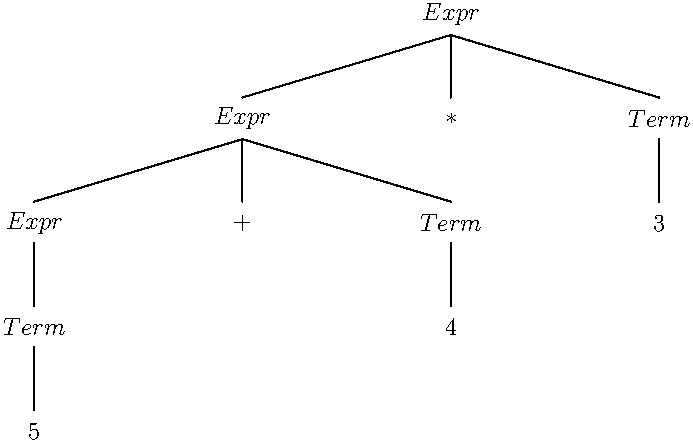
\includegraphics[width=15cm]{p1.pdf}
\caption{DFSA of keywords in Clite}
\label{p1}
\end{center}
\end{figure}

\section*{Problem 6}
\textbf{Q:} \textit{C and C++ distinguish between declarations and definitions. What is the distinction? Give an example of each each.}

\begin{itemize}
\item In C, we could write ``foo;'' -- this means we declare a integer variable ``foo'', if not declared before.
\item In C++, if we write ``foo'' and it is not declared, the compiler will return an error. We must write ``int foo;'' instead.
\end{itemize}

\section*{Problem 8}
\textbf{Q:} \textit{For the language C, give three examples of r-values that cannot be l-values. Give three more examples of l-values? Are there l-values that cannot be r-values? Explain.}

The first example that r-values cannot be l-values is:
\begin{lstlisting}
int a;
a = 25;
\end{lstlisting}

In this case, r-value ``25'' cannot be a l-value.

The second example is:
\begin{lstlisting}
int a;
const int b = 100;
a = b;
\end{lstlisting}

Here constant ``b'' should not be a l-value.

And now the third:
\begin{lstlisting}
int a, b = 0;
a = (++b);
\end{lstlisting}

The expression ``++b'' can't be l-value.

But all l-values could be r-values, so there is not an example that l-values cannot be r-values.

\section*{Problem 9}
\textbf{Q:} \textit{For the snippet of C++ codes: a) Using static scoping, write down the symbol table stacks at line 5, 12 and 20. b) Using dynamic scoping, write down the symbol table stacks at line 5 for call histories: main(28) $\rightarrow$ A(19) $\rightarrow$ B(11) $\rightarrow$ C, main(28) $\rightarrow$ B(11) $\rightarrow$ C}

The symbol tables are shown in tables below.

\begin{table}[hp]
\begin{center}
\begin{tabular}{l}
\toprule
\multicolumn{1}{c}{Symbol Stack}\\
\midrule
\textless var1, 2\textgreater\ \textless m, 4\textgreater\ \textless n, 4\textgreater\ \textless l, 4\textgreater \\
\textless x, 1\textgreater\ \textless y, 1\textgreater\ \textless z, 1\textgreater\ \textless C, 2\textgreater\ \textless b, 9\textgreater\ \textless a, 16\textgreater\ \textless main, 24\textgreater\\
\bottomrule
\end{tabular}
\caption{Symbol table with static scoping at line 5}
\end{center}
\end{table}

\begin{table}[hp]
\begin{center}
\begin{tabular}{l}
\toprule
\multicolumn{1}{c}{Symbol Stack}\\
\midrule
\textless var2, 9\textgreater\ \textless var3, 9\textgreater \\
\textless x, 1\textgreater\ \textless y, 1\textgreater\ \textless z, 1\textgreater\ \textless C, 2\textgreater\ \textless b, 9\textgreater\ \textless a, 16\textgreater\ \textless main, 24\textgreater\\
\bottomrule
\end{tabular}
\caption{Symbol table with static scoping at line 12}
\end{center}
\end{table}

\begin{table}[hp]
\begin{center}
\begin{tabular}{l}
\toprule
\multicolumn{1}{c}{Symbol Stack}\\
\midrule
\textless var4, 16\textgreater\ \textless var5, 16\textgreater\ \textless var6, 16\textgreater\ \textless z, 18\textgreater\ \textless w, 18\textgreater\ \textless u, 18\textgreater \\
\textless x, 1\textgreater\ \textless y, 1\textgreater\ \textless z, 1\textgreater\ \textless C, 2\textgreater\ \textless b, 9\textgreater\ \textless a, 16\textgreater\ \textless main, 24\textgreater\\
\bottomrule
\end{tabular}
\caption{Symbol table with static scoping at line 20}
\end{center}
\end{table}

\begin{table}[hp]
\begin{center}
\begin{tabular}{l}
\toprule
\multicolumn{1}{c}{Symbol Stack}\\
\midrule
\textless var1, 2\textgreater \\
\textless C, 2\textgreater \\
\textless var3, 9\textgreater\ \textless var2, 9\textgreater \\
\textless B, 9\textgreater \\
\textless z, 21\textgreater\ \textless var6, 16\textgreater\ \textless var5, 16\textgreater\ \textless var4, 16\textgreater \\
\textless A, 16\textgreater \\
\textless c, 27\textgreater\ \textless b, 27\textgreater\ \textless a, 27\textgreater\ \textless args, 24\textgreater \\
\textless main, 24\textgreater \\
\textless z, 1\textgreater\ \textless y, 1\textgreater\ \textless x, 1\textgreater \\
\bottomrule
\end{tabular}
\caption{Symbol table with dynamic scoping with first path}
\end{center}
\end{table}

\begin{table}[hp]
\begin{center}
\begin{tabular}{l l}
\toprule
\multicolumn{1}{c}{Symbol Stack}\\
\midrule
\textless var1, 2\textgreater \\
\textless C, 2\textgreater \\
\textless var3, 9\textgreater\ \textless var2, 9\textgreater \\
\textless B, 9\textgreater \\
\textless c, 27\textgreater\ \textless b, 27\textgreater\ \textless a, 27\textgreater\ \textless args, 24\textgreater \\
\textless main, 24\textgreater \\
\textless z, 1\textgreater\ \textless y, 1\textgreater\ \textless x, 1\textgreater \\
\bottomrule
\end{tabular}
\caption{Symbol table with dynamic scoping with second path}
\end{center}
\end{table}

\end{document}
